\documentclass{article}
\usepackage{amsmath}
\usepackage{amssymb}
\usepackage{array}
\usepackage{graphicx} % Required for \scalebox
\usepackage{hyperref}
\usepackage{listings}
\usepackage{xcolor}
\usepackage{graphicx}
\usepackage{booktabs}
\usepackage{verbatim}
\setcounter{MaxMatrixCols}{20}
\title{Baruch NLA HW4}
\author{Daniel Tuzes, 21}

\lstset{
    language=Python,
    basicstyle=\ttfamily\small,
    keywordstyle=\color{blue},
    commentstyle=\color{green!60!black},
    stringstyle=\color{orange},
    showstringspaces=false,
    breaklines=true,
    frame=single
}
\begin{document}
\maketitle
\section{Market Example from NLA Primer}

I will use python to construct and solve the equation $MQ=P_{t_0}$,
where $M$ is the payoff matrix,
$Q$ is the state price vector,
and $P_{t_0}$ is the price vector at $t_0$,
\[
    P_{t_0}^T = \begin{bmatrix} 46.6 & 51.55 & 63.3 & 95.3 & 99.55 & 84.9 & 47.25 & 15.8 & 7.9 \end{bmatrix}
\]
\subsection{Payoff matrix with market states 800 and 1650}
\[
    \begin{bmatrix}
        375 & 0     & 0   & 0  & 0    & 0    & 0   & 0   & 0   \\
        400 & 12.5  & 0   & 0  & 0    & 0    & 0   & 0   & 0   \\
        450 & 62.5  & 25  & 0  & 0    & 0    & 0   & 0   & 0   \\
        550 & 162.5 & 125 & 50 & 0    & 0    & 0   & 0   & 0   \\
        0   & 0     & 0   & 0  & 12.5 & 62.5 & 150 & 225 & 300 \\
        0   & 0     & 0   & 0  & 0    & 37.5 & 125 & 200 & 275 \\
        0   & 0     & 0   & 0  & 0    & 0    & 50  & 125 & 200 \\
        0   & 0     & 0   & 0  & 0    & 0    & 0   & 25  & 100 \\
        0   & 0     & 0   & 0  & 0    & 0    & 0   & 0   & 50  \\
    \end{bmatrix}
\]

State price vector transposed: \[
    \begin{bmatrix} 0.1243 & 0.1475 & -0.0735 & 0.2435 & 0.106 & 0.062 & 0.313 & 0& 0.158 \end{bmatrix}
\]

Arbitrage free, i.e. all non-negative? False

\subsection{Payoff matrix with market states 800 and 1700}
\[
    \begin{bmatrix}
        375 & 0     & 0   & 0  & 0    & 0    & 0   & 0   & 0   \\
        400 & 12.5  & 0   & 0  & 0    & 0    & 0   & 0   & 0   \\
        450 & 62.5  & 25  & 0  & 0    & 0    & 0   & 0   & 0   \\
        550 & 162.5 & 125 & 50 & 0    & 0    & 0   & 0   & 0   \\
        0   & 0     & 0   & 0  & 12.5 & 62.5 & 150 & 225 & 350 \\
        0   & 0     & 0   & 0  & 0    & 37.5 & 125 & 200 & 325 \\
        0   & 0     & 0   & 0  & 0    & 0    & 50  & 125 & 250 \\
        0   & 0     & 0   & 0  & 0    & 0    & 0   & 25  & 150 \\
        0   & 0     & 0   & 0  & 0    & 0    & 0   & 0   & 100 \\
    \end{bmatrix}
\]

State price vector transposed:
\[
    P^T = \begin{bmatrix} 0.0095 & 0.0393 & 0.0813 & 0.275 & 0.246 & 0.1807 & 0.0947 & 0.0217 \end{bmatrix}
\]


Arbitrage free, i.e. all non-negative? False

\subsection{Payoff matrix with market states 800 and 1800}
\[
    \begin{bmatrix}
        375 & 0     & 0   & 0  & 0    & 0    & 0   & 0   & 0   \\
        400 & 12.5  & 0   & 0  & 0    & 0    & 0   & 0   & 0   \\
        450 & 62.5  & 25  & 0  & 0    & 0    & 0   & 0   & 0   \\
        550 & 162.5 & 125 & 50 & 0    & 0    & 0   & 0   & 0   \\
        0   & 0     & 0   & 0  & 12.5 & 62.5 & 150 & 225 & 450 \\
        0   & 0     & 0   & 0  & 0    & 37.5 & 125 & 200 & 425 \\
        0   & 0     & 0   & 0  & 0    & 0    & 50  & 125 & 350 \\
        0   & 0     & 0   & 0  & 0    & 0    & 0   & 25  & 250 \\
        0   & 0     & 0   & 0  & 0    & 0    & 0   & 0   & 200 \\
    \end{bmatrix}
\]

State price vector transposed: \[
    \begin{bmatrix} 0.1243 & 0.1475 & -0.0735 & 0.2435 & -0.131 & 0.299 & 0.076 & 0.237 & 0.0395 \end{bmatrix}
\]

Arbitrage free, i.e. all non-negative? False

\subsection{Payoff matrix with market states 950 and 1650}
\[
    \begin{bmatrix}
        225 & 0     & 0   & 0  & 0    & 0    & 0   & 0   & 0   \\
        250 & 12.5  & 0   & 0  & 0    & 0    & 0   & 0   & 0   \\
        300 & 62.5  & 25  & 0  & 0    & 0    & 0   & 0   & 0   \\
        400 & 162.5 & 125 & 50 & 0    & 0    & 0   & 0   & 0   \\
        0   & 0     & 0   & 0  & 12.5 & 62.5 & 150 & 225 & 300 \\
        0   & 0     & 0   & 0  & 0    & 37.5 & 125 & 200 & 275 \\
        0   & 0     & 0   & 0  & 0    & 0    & 50  & 125 & 200 \\
        0   & 0     & 0   & 0  & 0    & 0    & 0   & 25  & 100 \\
        0   & 0     & 0   & 0  & 0    & 0    & 0   & 0   & 50  \\
    \end{bmatrix}
\]

State price vector transposed: \[
    \begin{bmatrix} 0.2071 & -0.0182 & 0.0922 & 0.0778 & 0.106 & 0.062 & 0.313 & 0& 0.158 \end{bmatrix}
\]

Arbitrage free, i.e. all non-negative? False

\subsection{Payoff matrix with market states 950 and 1700}
\[
    \begin{bmatrix}
        225 & 0     & 0   & 0  & 0    & 0    & 0   & 0   & 0   \\
        250 & 12.5  & 0   & 0  & 0    & 0    & 0   & 0   & 0   \\
        300 & 62.5  & 25  & 0  & 0    & 0    & 0   & 0   & 0   \\
        400 & 162.5 & 125 & 50 & 0    & 0    & 0   & 0   & 0   \\
        0   & 0     & 0   & 0  & 12.5 & 62.5 & 150 & 225 & 350 \\
        0   & 0     & 0   & 0  & 0    & 37.5 & 125 & 200 & 325 \\
        0   & 0     & 0   & 0  & 0    & 0    & 50  & 125 & 250 \\
        0   & 0     & 0   & 0  & 0    & 0    & 0   & 25  & 150 \\
        0   & 0     & 0   & 0  & 0    & 0    & 0   & 0   & 100 \\
    \end{bmatrix}
\]

State price vector transposed: \[
    \begin{bmatrix} 0.2071 & -0.0182 & 0.0922 & 0.0778 & -0.052 & 0.22 & 0.155 & 0.158 & 0.079 \end{bmatrix}
\]

Arbitrage free, i.e. all non-negative? False

\subsection{Payoff matrix with market states 950 and 1800}
\[
    \begin{bmatrix}
        225 & 0     & 0   & 0  & 0    & 0    & 0   & 0   & 0   \\
        250 & 12.5  & 0   & 0  & 0    & 0    & 0   & 0   & 0   \\
        300 & 62.5  & 25  & 0  & 0    & 0    & 0   & 0   & 0   \\
        400 & 162.5 & 125 & 50 & 0    & 0    & 0   & 0   & 0   \\
        0   & 0     & 0   & 0  & 12.5 & 62.5 & 150 & 225 & 450 \\
        0   & 0     & 0   & 0  & 0    & 37.5 & 125 & 200 & 425 \\
        0   & 0     & 0   & 0  & 0    & 0    & 50  & 125 & 350 \\
        0   & 0     & 0   & 0  & 0    & 0    & 0   & 25  & 250 \\
        0   & 0     & 0   & 0  & 0    & 0    & 0   & 0   & 200 \\
    \end{bmatrix}
\]

State price vector transposed: \[
    \begin{bmatrix} 0.2071 & -0.0182 & 0.0922 & 0.0778 & -0.131 & 0.299 & 0.076 & 0.237 & 0.0395 \end{bmatrix}
\]

Arbitrage free, i.e. all non-negative? False

\subsection{Payoff matrix with market states 1100 and 1650}
\[
    \begin{bmatrix}
        75  & 0     & 0   & 0  & 0    & 0    & 0   & 0   & 0   \\
        100 & 12.5  & 0   & 0  & 0    & 0    & 0   & 0   & 0   \\
        150 & 62.5  & 25  & 0  & 0    & 0    & 0   & 0   & 0   \\
        250 & 162.5 & 125 & 50 & 0    & 0    & 0   & 0   & 0   \\
        0   & 0     & 0   & 0  & 12.5 & 62.5 & 150 & 225 & 300 \\
        0   & 0     & 0   & 0  & 0    & 37.5 & 125 & 200 & 275 \\
        0   & 0     & 0   & 0  & 0    & 0    & 50  & 125 & 200 \\
        0   & 0     & 0   & 0  & 0    & 0    & 0   & 25  & 100 \\
        0   & 0     & 0   & 0  & 0    & 0    & 0   & 0   & 50  \\
    \end{bmatrix}
\]

State price vector transposed: \[
    \begin{bmatrix} 0.6213 & -0.8467 & 0.9207 & -0.7507 & 0.106 & 0.062 & 0.313 & 0& 0.158 \end{bmatrix}
\]

Arbitrage free, i.e. all non-negative? False

\subsection{Payoff matrix with market states 1100 and 1700}
\[
    \begin{bmatrix}
        75  & 0     & 0   & 0  & 0    & 0    & 0   & 0   & 0   \\
        100 & 12.5  & 0   & 0  & 0    & 0    & 0   & 0   & 0   \\
        150 & 62.5  & 25  & 0  & 0    & 0    & 0   & 0   & 0   \\
        250 & 162.5 & 125 & 50 & 0    & 0    & 0   & 0   & 0   \\
        0   & 0     & 0   & 0  & 12.5 & 62.5 & 150 & 225 & 350 \\
        0   & 0     & 0   & 0  & 0    & 37.5 & 125 & 200 & 325 \\
        0   & 0     & 0   & 0  & 0    & 0    & 50  & 125 & 250 \\
        0   & 0     & 0   & 0  & 0    & 0    & 0   & 25  & 150 \\
        0   & 0     & 0   & 0  & 0    & 0    & 0   & 0   & 100 \\
    \end{bmatrix}
\]

State price vector transposed: \[
    \begin{bmatrix} 0.6213 & -0.8467 & 0.9207 & -0.7507 & -0.052 & 0.22 & 0.155 & 0.158 & 0.079 \end{bmatrix}
\]

Arbitrage free, i.e. all non-negative? False

\subsection{Payoff matrix with market states 1100 and 1800}
\[
    \begin{bmatrix}
        75  & 0     & 0   & 0  & 0    & 0    & 0   & 0   & 0   \\
        100 & 12.5  & 0   & 0  & 0    & 0    & 0   & 0   & 0   \\
        150 & 62.5  & 25  & 0  & 0    & 0    & 0   & 0   & 0   \\
        250 & 162.5 & 125 & 50 & 0    & 0    & 0   & 0   & 0   \\
        0   & 0     & 0   & 0  & 12.5 & 62.5 & 150 & 225 & 450 \\
        0   & 0     & 0   & 0  & 0    & 37.5 & 125 & 200 & 425 \\
        0   & 0     & 0   & 0  & 0    & 0    & 50  & 125 & 350 \\
        0   & 0     & 0   & 0  & 0    & 0    & 0   & 25  & 250 \\
        0   & 0     & 0   & 0  & 0    & 0    & 0   & 0   & 200 \\
    \end{bmatrix}
\]

State price vector transposed: \[
    \begin{bmatrix} 0.6213 & -0.8467 & 0.9207 & -0.7507 & -0.131 & 0.299 & 0.076 & 0.237 & 0.0395 \end{bmatrix}
\]

Arbitrage free, i.e. all non-negative? False

\section{Neftci’s Financial Engineering book}

First I find the instruments and define the payoff matrix.
See them in \autoref{neftci_first}.
Given a payoff matrix \( M \) and a price vector \( P \),
I seek to find the state prices vector \( Q \)
that satisfies the equation: \(M \cdot Q = P\). Here

\[
    M = \begin{bmatrix}
        150 & 0   & 0  & 0    & 0     & 0   \\
        300 & 75  & 0  & 0    & 0     & 0   \\
        450 & 225 & 75 & 0    & 0     & 0   \\
        0   & 0   & 0  & 37.5 & 112.5 & 200 \\
        0   & 0   & 0  & 0    & 37.5  & 125 \\
        0   & 0   & 0  & 0    & 0     & 50
    \end{bmatrix},
    \quad P = \begin{bmatrix}
        3.75  \\
        14.75 \\
        54.9  \\
        53.8  \\
        22.3  \\
        6.8
    \end{bmatrix}
\]
Solving this system of linear equations yields: \[
    Q^T = \begin{bmatrix}
        0.025 & 0.0967 & 0.292 & 0.2853 & 0.1413 & 0.136
    \end{bmatrix}
\]
The payoff matrix for the reaminaing options are in \autoref{payoff_reaminaing}.
Given the state price vector \( Q \) and the payoff matrix \( M \) for the options,
the interpolated price \( \hat{P} \) for each option can be calculated as follows:
\[
    \hat{P}_i = \sum_{j=1}^{n} M_{ij} \cdot Q_j,
\]
where:
\begin{itemize}
    \item \( M_{ij} \) represents the payoff of the \( i \)-th option at the \( j \)-th market state.
    \item \( Q_j \) is the price of the \( j \)-th state, derived from solving \( MQ = P \).
    \item \( n \) is the total number of market states.
\end{itemize}

Some instruments have constant 0 payoff, their estimated price is 0.
The results are in \autoref{payoff_reaminaing},
at column Int and visualized in \autoref{fig:options_prices}.
The relative error is in column D.
Sum of Absolute Differences: 20.604.
We had total of 19 unfitted instruments and 6 used for the $Q$ calibration.
\begin{itemize}
    \item The mean taken over the new instruments only is $20.604/19 \approx 1.084$, and
    \item the mean taken over all the instruments is $20.604/25 \approx 0.824$.
\end{itemize}


\begin{table}[h]
    \centering
    \caption{Option payoffs at different market states in the first case\label{neftci_first}}
    \begin{tabular}{|c|c|c|c|c|c|c|c|c|}
        \hline
        \multicolumn{3}{|c|}{\textbf{Option}} & \multicolumn{6}{c|}{$\omega$}                                                              \\ \hline
        \textbf{Type}                         & \textbf{Strike}               & \textbf{Price} & 750 & 975 & 1125 & 1237.5 & 1312.5 & 1400 \\ \hline
        Put                                   & 900                           & 3.75           & 150 & 0   & 0    & 0      & 0      & 0    \\ \hline
        Put                                   & 1050                          & 14.75          & 300 & 75  & 0    & 0      & 0      & 0    \\ \hline
        Put                                   & 1200                          & 54.9           & 450 & 225 & 75   & 0      & 0      & 0    \\ \hline
        Call                                  & 1200                          & 53.8           & 0   & 0   & 0    & 37.5   & 112.5  & 200  \\ \hline
        Call                                  & 1275                          & 22.3           & 0   & 0   & 0    & 0      & 37.5   & 125  \\ \hline
        Call                                  & 1350                          & 6.8            & 0   & 0   & 0    & 0      & 0      & 50   \\ \hline
    \end{tabular}
\end{table}

\begin{table}[h]
    \centering
    \caption{\label{payoff_reaminaing}
        Payoff matrix for the remaining options.
        Mid is the mid price of ask and bid,
        Int is the calculated price from the payoff matrix and $Q$.
        D is the absolute value of relative difference, in percentage.}
    \small
    \begin{tabular}{lrrrrrrrrrrrr}
        \toprule
        T    & Str  & Bid  & Ask  & Mid   & 750 & 975 & 1125 & 1237.5 & 1312.5 & 1400 & Int   & D $\%$ \\
        \midrule
        Put  & 800  & 1.2  & 1.65 & 1.42  & 50  & 0   & 0    & 0.     & 0.     & 0    & 1.25  & 12.28  \\
        Put  & 950  & 5.3  & 6.3  & 5.8   & 200 & 0   & 0    & 0.     & 0.     & 0    & 5.    & 13.79  \\
        Put  & 995  & 8.5  & 9.5  & 9.    & 245 & 20  & 0    & 0.     & 0.     & 0    & 8.06  & 10.46  \\
        Put  & 1025 & 11.1 & 12.6 & 11.85 & 275 & 50  & 0    & 0.     & 0.     & 0    & 11.71 & 1.2    \\
        Put  & 1060 & 15.7 & 17.2 & 16.45 & 310 & 85  & 0    & 0.     & 0.     & 0    & 15.97 & 2.94   \\
        Put  & 1075 & 18.  & 19.5 & 18.75 & 325 & 100 & 0    & 0.     & 0.     & 0    & 17.79 & 5.11   \\
        Put  & 1100 & 22.7 & 24.7 & 23.7  & 350 & 125 & 0    & 0.     & 0.     & 0    & 20.83 & 12.1   \\
        Put  & 1150 & 35.3 & 37.3 & 36.3  & 400 & 175 & 25   & 0.     & 0.     & 0    & 34.22 & 5.74   \\
        Put  & 1175 & 44.1 & 46.1 & 45.1  & 425 & 200 & 50   & 0.     & 0.     & 0    & 44.56 & 1.2    \\
        Call & 1175 & 68.  & 70.  & 69.   & 0   & 0   & 0    & 62.5   & 137.5  & 225  & 67.87 & 1.64   \\
        Call & 1225 & 40.3 & 42.3 & 41.3  & 0   & 0   & 0    & 12.5   & 87.5   & 175  & 39.73 & 3.79   \\
        Call & 1250 & 29.6 & 31.6 & 30.6  & 0   & 0   & 0    & 0.     & 62.5   & 150  & 29.23 & 4.47   \\
        Call & 1300 & 15.  & 16.2 & 15.6  & 0   & 0   & 0    & 0.     & 12.5   & 100  & 15.37 & 1.5    \\
        Call & 1325 & 10.  & 11.  & 10.5  & 0   & 0   & 0    & 0.     & 0.     & 75   & 10.2  & 2.86   \\
        Call & 1375 & 4.   & 4.7  & 4.35  & 0   & 0   & 0    & 0.     & 0.     & 25   & 3.4   & 21.84  \\
        Call & 1400 & 2.5  & 3.2  & 2.85  & 0   & 0   & 0    & 0.     & 0.     & 0    & 0.    & 100.   \\
        Call & 1425 & 1.4  & 1.85 & 1.62  & 0   & 0   & 0    & 0.     & 0.     & 0    & 0.    & 100.   \\
        Call & 1450 & 0.8  & 1.25 & 1.02  & 0   & 0   & 0    & 0.     & 0.     & 0    & 0.    & 100.   \\
        Call & 1475 & 0.35 & 0.8  & 0.57  & 0   & 0   & 0    & 0.     & 0.     & 0    & 0.    & 100.   \\
        \bottomrule
    \end{tabular}


\end{table}

\begin{figure}[htbp]
    \centering
    \caption{Comparison of market and interpolated prices
        for the first market from Neftci's
        \label{fig:options_prices}}
    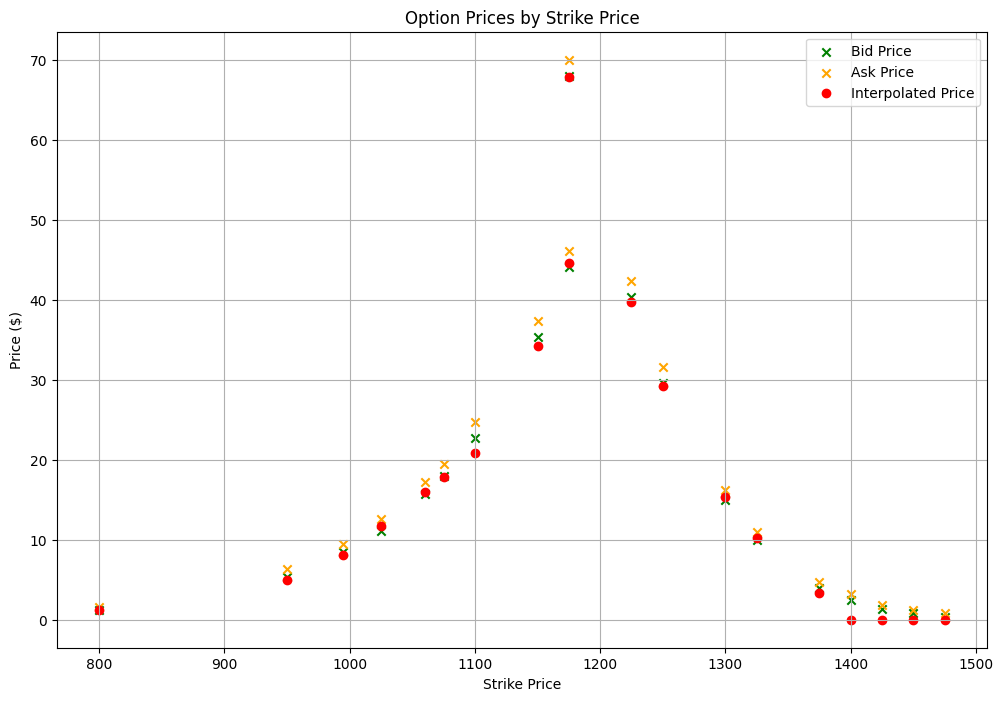
\includegraphics[width=\linewidth]{output.pdf}
\end{figure}

\subsection{New market}
The properties of the new options defining the market are in \autoref{newopt}.
\begin{table}
    \centering
    \caption{New options defining new market\label{newopt}}
    \begin{tabular}{lrrrr}
        \toprule
        Type & Strike & Ask  & Bid  & Mid Price \\
        \midrule
        Put  & 800    & 1.65 & 1.2  & 1.42      \\
        Put  & 950    & 6.3  & 5.3  & 5.8       \\
        Put  & 1050   & 15.5 & 14   & 14.75     \\
        Put  & 1200   & 55.9 & 53.9 & 54.9      \\
        Call & 1200   & 54.8 & 52.8 & 53.8      \\
        Call & 1275   & 23.3 & 21.3 & 22.3      \\
        Call & 1350   & 7.3  & 6.3  & 6.8       \\
        Call & 1425   & 1.85 & 1.4  & 1.62      \\
        \bottomrule
    \end{tabular}
\end{table}

The payoff matrix is defined in \autoref{newpayoff}.

\begin{table}
    \centering
    \caption{Payoff matrix for the new options at the new market states \label{newpayoff}}
    \begin{tabular}{lrrrrrrrr}
        \toprule
                  & 650 & 875 & 1000 & 1125 & 1237.5 & 1312.5 & 1387.5 & 1500 \\
        \midrule
        800 Put   & 150 & 0   & 0    & 0    & 0      & 0      & 0      & 0    \\
        950 Put   & 300 & 75  & 0    & 0    & 0      & 0      & 0      & 0    \\
        1050 Put  & 400 & 175 & 50   & 0    & 0      & 0      & 0      & 0    \\
        1200 Put  & 550 & 325 & 200  & 75   & 0      & 0      & 0      & 0    \\
        1200 Call & 0   & 0   & 0    & 0    & 37.5   & 112.5  & 187.5  & 300  \\
        1275 Call & 0   & 0   & 0    & 0    & 0      & 37.5   & 112.5  & 225  \\
        1350 Call & 0   & 0   & 0    & 0    & 0      & 0      & 37.5   & 150  \\
        1425 Call & 0   & 0   & 0    & 0    & 0      & 0      & 0      & 75   \\
        \bottomrule
    \end{tabular}
\end{table}

With \verb|np.linalg.matrix_rank| we can check that the rank for the payoff matrix is 8,
so the securities are non-redundant and the market is complete.


Given the matrix \( M \) (payoff matrix)
and vector \( P \)(price vector),
the relationship between the state prices \( Q \) is given by \(MQ = P\),
where:
\[
    M = \begin{bmatrix}
        150 & 0   & 0   & 0  & 0    & 0     & 0     & 0     \\
        300 & 75  & 0   & 0  & 0    & 0     & 0     & 0     \\
        400 & 175 & 50  & 0  & 0    & 0     & 0     & 0     \\
        550 & 325 & 200 & 75 & 0    & 0     & 0     & 0     \\
        0   & 0   & 0   & 0  & 37.5 & 112.5 & 187.5 & 300   \\
        0   & 0   & 0   & 0  & 0    & 37.5  & 112.5 & 225   \\
        0   & 0   & 0   & 0  & 0    & 0     & 37.5  & 150   \\
        0   & 0   & 0   & 0  & 0    & 0     & 0     & 75.00
    \end{bmatrix},
    \quad P = \begin{bmatrix}
        1.42  \\
        5.8   \\
        14.75 \\
        54.9  \\
        53.8  \\
        22.3  \\
        6.8   \\
        1.62
    \end{bmatrix}
\]
With \verb|np.linalg.solve| the solution is
\[
    Q^T = \begin{bmatrix} 0.0095 & 0.0393 & 0.0813 & 0.275 & 0.246 & 0.1807 & 0.0947 & 0.0217 \end{bmatrix}
\]

\subsection*{pricing other instruments}
The other isntruments are

\begin{tabular}{lrrrr}
    \toprule
    Type & Strike & Bid  & Ask  & Mid Price \\
    \midrule
    Put  & 900    & 3.4  & 4.1  & 3.75      \\
    Put  & 995    & 8.5  & 9.5  & 9.        \\
    Put  & 1025   & 11.1 & 12.6 & 11.85     \\
    Put  & 1060   & 15.7 & 17.2 & 16.45     \\
    Put  & 1075   & 18.  & 19.5 & 18.75     \\
    Put  & 1100   & 22.7 & 24.7 & 23.7      \\
    Put  & 1150   & 35.3 & 37.3 & 36.3      \\
    Put  & 1175   & 44.1 & 46.1 & 45.1      \\
    Call & 1175   & 68.  & 70.  & 69.       \\
    Call & 1225   & 40.3 & 42.3 & 41.3      \\
    Call & 1250   & 29.6 & 31.6 & 30.6      \\
    Call & 1300   & 15.  & 16.2 & 15.6      \\
    Call & 1325   & 10.  & 11.  & 10.5      \\
    Call & 1375   & 4.   & 4.7  & 4.35      \\
    Call & 1400   & 2.5  & 3.2  & 2.85      \\
    Call & 1450   & 0.8  & 1.25 & 1.02      \\
    Call & 1475   & 0.35 & 0.8  & 0.57      \\
    \bottomrule
\end{tabular}

They define the payoff matrix

\begin{tabular}{lrrrrrrrr}
    \toprule
              & 650 & 875 & 1000 & 1125 & 1237.5 & 1312.5 & 1387.5 & 1500 \\
    \midrule
    900 Put   & 250 & 25  & 0    & 0    & 0      & 0      & 0      & 0    \\
    995 Put   & 345 & 120 & 0    & 0    & 0      & 0      & 0      & 0    \\
    1025 Put  & 375 & 150 & 25   & 0    & 0      & 0      & 0      & 0    \\
    1060 Put  & 410 & 185 & 60   & 0    & 0      & 0      & 0      & 0    \\
    1075 Put  & 425 & 200 & 75   & 0    & 0      & 0      & 0      & 0    \\
    1100 Put  & 450 & 225 & 100  & 0    & 0      & 0      & 0      & 0    \\
    1150 Put  & 500 & 275 & 150  & 25   & 0      & 0      & 0      & 0    \\
    1175 Put  & 525 & 300 & 175  & 50   & 0      & 0      & 0      & 0    \\
    1175 Call & 0   & 0   & 0    & 0    & 62     & 138    & 212    & 325  \\
    1225 Call & 0   & 0   & 0    & 0    & 12     & 88     & 162    & 275  \\
    1250 Call & 0   & 0   & 0    & 0    & 0      & 62     & 138    & 250  \\
    1300 Call & 0   & 0   & 0    & 0    & 0      & 12     & 88     & 200  \\
    1325 Call & 0   & 0   & 0    & 0    & 0      & 0      & 62     & 175  \\
    1375 Call & 0   & 0   & 0    & 0    & 0      & 0      & 12     & 125  \\
    1400 Call & 0   & 0   & 0    & 0    & 0      & 0      & 0      & 100  \\
    1450 Call & 0   & 0   & 0    & 0    & 0      & 0      & 0      & 50   \\
    1475 Call & 0   & 0   & 0    & 0    & 0      & 0      & 0      & 25   \\
    \bottomrule
\end{tabular}



The new prices using the $P=MQ$ formula:

\begin{tabular}{lrrrrrr}
    \toprule
    Type & Strike & Bid   & Ask   & Mid Price & Estimated Price & D $\%$ \\
    \midrule
    Put  & 900    & 3.40  & 4.10  & 3.75      & 3.36            & 10.44  \\
    Put  & 995    & 8.50  & 9.50  & 9.00      & 8.00            & 11.14  \\
    Put  & 1025   & 11.10 & 12.60 & 11.85     & 11.50           & 2.99   \\
    Put  & 1060   & 15.70 & 17.20 & 16.45     & 16.05           & 2.42   \\
    Put  & 1075   & 18.00 & 19.50 & 18.75     & 18.00           & 3.98   \\
    Put  & 1100   & 22.70 & 24.70 & 23.70     & 21.26           & 10.30  \\
    Put  & 1150   & 35.30 & 37.30 & 36.30     & 34.64           & 4.57   \\
    Put  & 1175   & 44.10 & 46.10 & 45.10     & 44.77           & 0.73   \\
    Call & 1175   & 68.00 & 70.00 & 69.00     & 67.38           & 2.36   \\
    Call & 1225   & 40.30 & 42.30 & 41.30     & 40.22           & 2.60   \\
    Call & 1250   & 29.60 & 31.60 & 30.60     & 29.72           & 2.86   \\
    Call & 1300   & 15.00 & 16.20 & 15.60     & 14.88           & 4.65   \\
    Call & 1325   & 10.00 & 11.00 & 10.50     & 9.71            & 7.54   \\
    Call & 1375   & 4.00  & 4.70  & 4.35      & 3.89            & 10.54  \\
    Call & 1400   & 2.50  & 3.20  & 2.85      & 2.17            & 23.98  \\
    Call & 1450   & 0.80  & 1.25  & 1.02      & 1.08            & 5.69   \\
    Call & 1475   & 0.35  & 0.80  & 0.57      & 0.54            & 5.80   \\
    \bottomrule
\end{tabular}





The absolute difference is $13.64$.
\begin{itemize}
    \item We have 17 new instruments, the average is $0.803$, and
    \item over all instruments, 25, the average is $0.546$.
\end{itemize}


The results are visualized in \autoref{fig:options_prices2}.


\begin{figure}[htbp]
    \centering
    \caption{Comparison of market and interpolated prices
        for the 2nd, extended market from Neftci's
        \label{fig:options_prices2}}
    \includegraphics[width=\linewidth]{output2.pdf}
\end{figure}


\end{document}